\documentclass{standalone}
\usepackage{tikz}
\usetikzlibrary{patterns, positioning}


\begin{document}
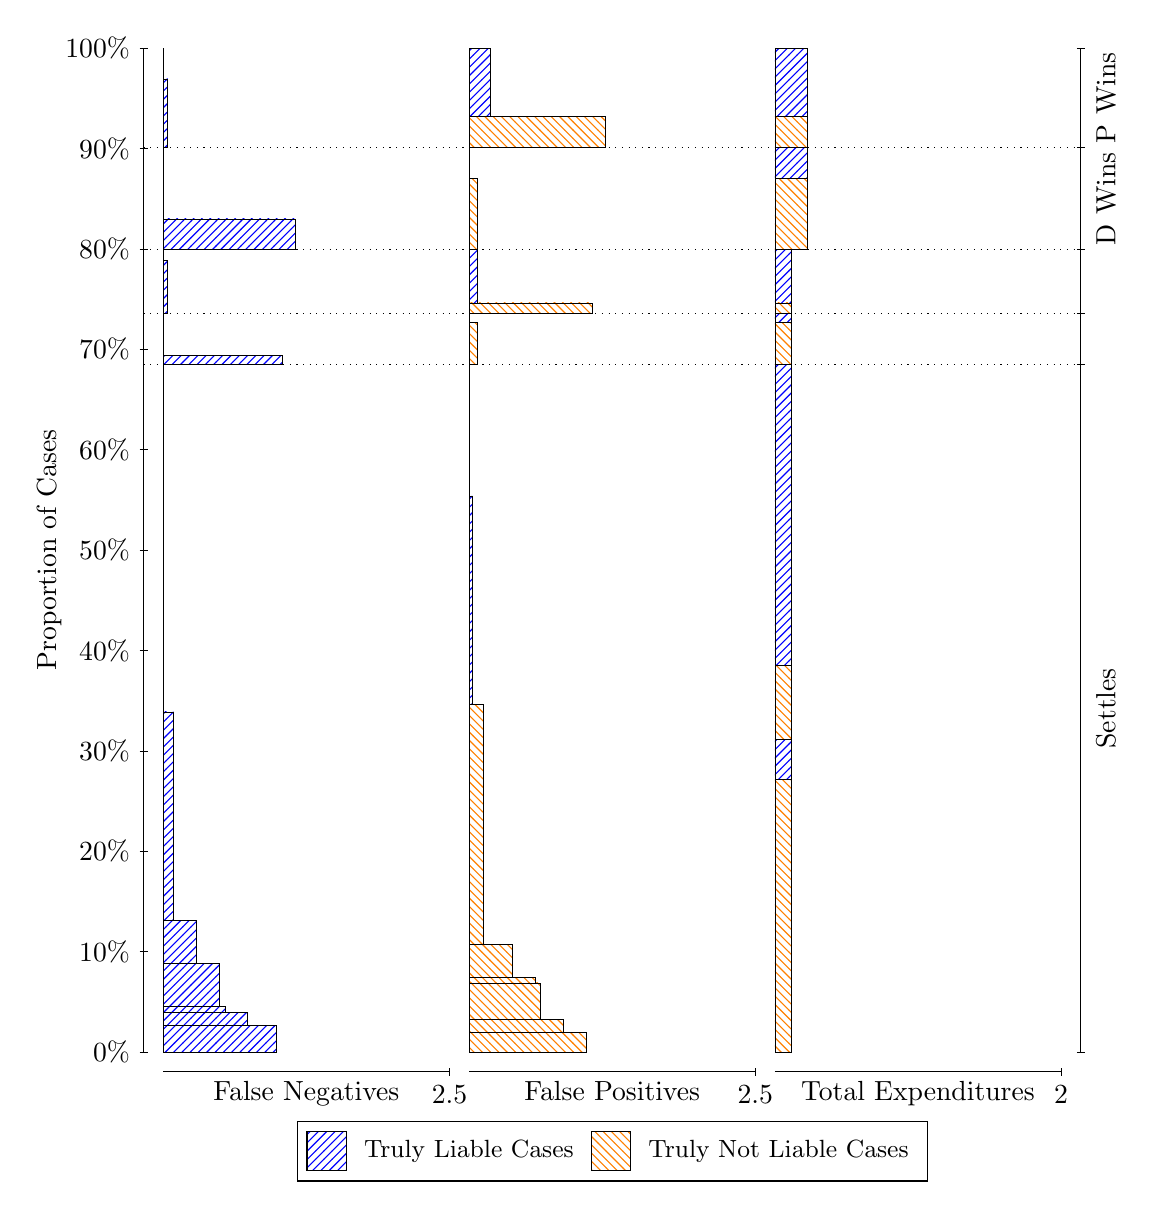
\begin{tikzpicture}
\draw[black, very thin] (1.5,1.75) -- (1.5,14.5);
\node[rotate=90, text=black, anchor=center] at (0.3, 8.125) {Proportion of Cases};
\draw[black, very thin] (1.45,1.75) -- (1.55,1.75);
\node[text=black, anchor=east] at (1.45, 1.75) {0\%};
\draw[black, very thin] (1.45,3.025) -- (1.55,3.025);
\node[text=black, anchor=east] at (1.45, 3.025) {10\%};
\draw[black, very thin] (1.45,4.3) -- (1.55,4.3);
\node[text=black, anchor=east] at (1.45, 4.3) {20\%};
\draw[black, very thin] (1.45,5.575) -- (1.55,5.575);
\node[text=black, anchor=east] at (1.45, 5.575) {30\%};
\draw[black, very thin] (1.45,6.85) -- (1.55,6.85);
\node[text=black, anchor=east] at (1.45, 6.85) {40\%};
\draw[black, very thin] (1.45,8.125) -- (1.55,8.125);
\node[text=black, anchor=east] at (1.45, 8.125) {50\%};
\draw[black, very thin] (1.45,9.4) -- (1.55,9.4);
\node[text=black, anchor=east] at (1.45, 9.4) {60\%};
\draw[black, very thin] (1.45,10.675) -- (1.55,10.675);
\node[text=black, anchor=east] at (1.45, 10.675) {70\%};
\draw[black, very thin] (1.45,11.95) -- (1.55,11.95);
\node[text=black, anchor=east] at (1.45, 11.95) {80\%};
\draw[black, very thin] (1.45,13.225) -- (1.55,13.225);
\node[text=black, anchor=east] at (1.45, 13.225) {90\%};
\draw[black, very thin] (1.45,14.5) -- (1.55,14.5);
\node[text=black, anchor=east] at (1.45, 14.5) {100\%};

\draw[black, very thin] (13.4,1.75) -- (13.4,14.5);
\draw[black, very thin] (13.35,1.75) -- (13.45,1.75);
\node[anchor=west] at (13.35, 1.75) {};
\draw[black, very thin] (13.35,10.478) -- (13.45,10.478);
\node[anchor=west] at (13.35, 10.478) {};
\draw[black, very thin] (13.35,11.133) -- (13.45,11.133);
\node[anchor=west] at (13.35, 11.133) {};
\draw[black, very thin] (13.35,11.939) -- (13.45,11.939);
\node[anchor=west] at (13.35, 11.939) {};
\draw[black, very thin] (13.35,13.236) -- (13.45,13.236);
\node[anchor=west] at (13.35, 13.236) {};
\draw[black, very thin] (13.35,14.5) -- (13.45,14.5);
\node[anchor=west] at (13.35, 14.5) {};

\draw[black, very thin, pattern color=blue, pattern=north east lines] (1.75,1.75) rectangle (3.1852,2.0892);
\draw[black, very thin, pattern color=blue, pattern=north east lines] (1.75,2.0892) rectangle (2.8218,2.254);
\draw[black, very thin, pattern color=blue, pattern=north east lines] (1.75,2.254) rectangle (2.5312,2.3334);
\draw[black, very thin, pattern color=blue, pattern=north east lines] (1.75,2.3334) rectangle (2.4585,2.8707);
\draw[black, very thin, pattern color=blue, pattern=north east lines] (1.75,2.8707) rectangle (2.1678,3.4171);
\draw[black, very thin, pattern color=blue, pattern=north east lines] (1.75,3.4171) rectangle (1.8772,6.0684);
\draw[black, very thin, pattern color=orange, pattern=north west lines] (1.75,6.0684) rectangle (1.75,10.478);
\draw[black, very thin, pattern color=blue, pattern=north east lines] (1.75,10.478) rectangle (3.2578,10.595);
\draw[black, very thin, pattern color=orange, pattern=north west lines] (1.75,10.595) rectangle (1.75,11.133);
\draw[black, very thin, pattern color=blue, pattern=north east lines] (1.75,11.133) rectangle (1.8045,11.809);
\draw[black, very thin, pattern color=orange, pattern=north west lines] (1.75,11.809) rectangle (1.75,11.939);
\draw[black, very thin, pattern color=blue, pattern=north east lines] (1.75,11.939) rectangle (3.4213,12.331);
\draw[black, very thin, pattern color=orange, pattern=north west lines] (1.75,12.331) rectangle (1.75,13.236);
\draw[black, very thin, pattern color=blue, pattern=north east lines] (1.75,13.236) rectangle (1.8045,14.108);
\draw[black, very thin, pattern color=orange, pattern=north west lines] (1.75,14.108) rectangle (1.75,14.5);
\draw[black, very thin, pattern color=orange, pattern=north west lines] (5.6333,1.75) rectangle (7.123,2.0037);
\draw[black, very thin, pattern color=orange, pattern=north west lines] (5.6333,2.0037) rectangle (6.8323,2.166);
\draw[black, very thin, pattern color=orange, pattern=north west lines] (5.6333,2.166) rectangle (6.5417,2.627);
\draw[black, very thin, pattern color=orange, pattern=north west lines] (5.6333,2.627) rectangle (6.469,2.6955);
\draw[black, very thin, pattern color=orange, pattern=north west lines] (5.6333,2.6955) rectangle (6.1783,3.121);
\draw[black, very thin, pattern color=orange, pattern=north west lines] (5.6333,3.121) rectangle (5.815,6.1599);
\draw[black, very thin, pattern color=blue, pattern=north east lines] (5.6333,6.1599) rectangle (5.6697,8.8113);
\draw[black, very thin, pattern color=blue, pattern=north east lines] (5.6333,8.8113) rectangle (5.6333,10.478);
\draw[black, very thin, pattern color=orange, pattern=north west lines] (5.6333,10.478) rectangle (5.7423,11.016);
\draw[black, very thin, pattern color=blue, pattern=north east lines] (5.6333,11.016) rectangle (5.6333,11.133);
\draw[black, very thin, pattern color=orange, pattern=north west lines] (5.6333,11.133) rectangle (7.1957,11.263);
\draw[black, very thin, pattern color=blue, pattern=north east lines] (5.6333,11.263) rectangle (5.7423,11.939);
\draw[black, very thin, pattern color=orange, pattern=north west lines] (5.6333,11.939) rectangle (5.7423,12.844);
\draw[black, very thin, pattern color=blue, pattern=north east lines] (5.6333,12.844) rectangle (5.6333,13.236);
\draw[black, very thin, pattern color=orange, pattern=north west lines] (5.6333,13.236) rectangle (7.3592,13.628);
\draw[black, very thin, pattern color=blue, pattern=north east lines] (5.6333,13.628) rectangle (5.9058,14.5);
\draw[black, very thin, pattern color=orange, pattern=north west lines] (9.5167,1.75) rectangle (9.721,5.2144);
\draw[black, very thin, pattern color=blue, pattern=north east lines] (9.5167,5.2144) rectangle (9.721,5.7184);
\draw[black, very thin, pattern color=orange, pattern=north west lines] (9.5167,5.7184) rectangle (9.721,6.6639);
\draw[black, very thin, pattern color=blue, pattern=north east lines] (9.5167,6.6639) rectangle (9.721,10.478);
\draw[black, very thin, pattern color=orange, pattern=north west lines] (9.5167,10.478) rectangle (9.721,11.016);
\draw[black, very thin, pattern color=blue, pattern=north east lines] (9.5167,11.016) rectangle (9.721,11.133);
\draw[black, very thin, pattern color=orange, pattern=north west lines] (9.5167,11.133) rectangle (9.721,11.263);
\draw[black, very thin, pattern color=blue, pattern=north east lines] (9.5167,11.263) rectangle (9.721,11.939);
\draw[black, very thin, pattern color=orange, pattern=north west lines] (9.5167,11.939) rectangle (9.9254,12.844);
\draw[black, very thin, pattern color=blue, pattern=north east lines] (9.5167,12.844) rectangle (9.9254,13.236);
\draw[black, very thin, pattern color=orange, pattern=north west lines] (9.5167,13.236) rectangle (9.9254,13.628);
\draw[black, very thin, pattern color=blue, pattern=north east lines] (9.5167,13.628) rectangle (9.9254,14.5);
\draw[black, dotted] (1.5,10.478) -- (13.4,10.478);
\draw[black, dotted] (1.5,11.133) -- (13.4,11.133);
\draw[black, dotted] (1.5,11.939) -- (13.4,11.939);
\draw[black, dotted] (1.5,13.236) -- (13.4,13.236);
\draw[black, very thin] (1.75,1.5) -- (5.3833,1.5);
\node[text=black, anchor=north] at (3.5667, 1.5) {False Negatives};
\draw[black, very thin] (5.3833,1.45) -- (5.3833,1.55);
\node[text=black, anchor=north] at (5.3833, 1.45) {2.5};

\draw[black, very thin] (5.6333,1.5) -- (9.2667,1.5);
\node[text=black, anchor=north] at (7.45, 1.5) {False Positives};
\draw[black, very thin] (9.2667,1.45) -- (9.2667,1.55);
\node[text=black, anchor=north] at (9.2667, 1.45) {2.5};

\draw[black, very thin] (9.5167,1.5) -- (13.15,1.5);
\node[text=black, anchor=north] at (11.333, 1.5) {Total Expenditures};
\draw[black, very thin] (13.15,1.45) -- (13.15,1.55);
\node[text=black, anchor=north] at (13.15, 1.45) {2};

\node[text=black, centered, rotate=90] at (13.72, 6.1142) {Settles};


\node[text=black, centered, rotate=90] at (13.72, 12.587) {D Wins};
\node[text=black, centered, rotate=90] at (13.72, 13.868) {P Wins};

\draw (7.449999999999999,1.5) node[draw=none] (baseCoordinate) {};
\begin{scope}[align=center]
        \matrix[scale=0.5, draw=black, below=0.5cm of baseCoordinate, nodes={draw}, column sep=0.1cm]{
            \node[rectangle, draw, minimum width=0.5cm, minimum height=0.5cm, pattern color=blue, pattern=north east lines] {}; &
            \node[draw=none, font=\small, text=black] (B) {Truly Liable Cases}; &
            \node[rectangle, draw, minimum width=0.5cm, minimum height=0.5cm, pattern color=orange, pattern=north west lines] {}; &
            \node[draw=none, font=\small, text=black] (B) {Truly Not Liable Cases}; \\
            };
\end{scope}

\end{tikzpicture}
\end{document}